\documentclass[11pt]{beamer}
\usetheme{Warsaw}
\usepackage[utf8]{inputenc}
\usepackage[T1]{fontenc}
\usepackage{amsmath}
\usepackage{amsfonts}
\usepackage{amssymb}
\usepackage{graphicx}
\usepackage{subfig}
\usepackage[export]{adjustbox}
%%%%%%%%%%%%%%%%%%%%%%%%%%%%%%%%%%%%%%%%%%%%%%%%%%%%%%%%%%%%%%%%%%%%%%%%%%%%%%%%%5
\author{Fernando Del Fedele}
\title{Crecimiento y caracterización de
láminas delgadas con memoria de
forma de alta temperatura Ni-Ti-Zr
mediante sputtering.}
%\setbeamercovered{transparent} 
%\setbeamertemplate{navigation symbols}{} 
%\logo{} 
%\institute{} 
%\date{} 
%\subject{} 
\begin{document}

\begin{frame}
\titlepage
\end{frame}

\begin{frame}{Contenido}
\tableofcontents
\end{frame}

\section{Introducción}

\subsection{Objetivo}
	\subsection{Materiales con memoria de forma}
		\begin{frame}{Materiales con memoria de forma}
			Las aleaciones con memoria de forma, de aquí en adelante nombradas como \textbf{SMA} (del inglés, \textbf{S}hape \textbf{M}emory \textbf{A}lloys) son aleaciones que pueden recuperar su forma original al ser calentadas luego de haber sufrido una deformación aparentemente plástica
			Entre sus propiedades, se encuentran:
			\begin{itemize}
				\item Superelasticidad
				\item Alta capacidad de amortiguamiento
				\item Alta relación entre la potencia entregada y su peso
			\end{itemize}
		\end{frame}
		
	\subsection{Materiales con memoria de forma de alta temperatura}
		\begin{frame}
			Las aplicaciones actuales de los SMA están limitadas por debajo de los $100^\circ C$. Los materiales con memoria de forma de alta temperatura, abreviados como \textbf{HTSMA} (del inglés, \textbf{H}igh \textbf{T}emperature \textbf{S}hape \textbf{M}emory \textbf{A}lloys) son aquellos en los cuales la transformación martensítica sucede a $T > 100^\circ C$.
			
			Lo más común a es a $NiTi$ agregarle $Pd$ o $Pt$ en detrimento del $Ti$, pero recientemente se encontró que $Hf$ o $Zr$ tienen efectos aún mayores en la temperatura a menor costo relativo.
		\end{frame}
	
	\subsection{Transformación martensítica}
		\begin{frame}{Transformación martensítica}
			La causa del efecto de memoria de forma es la transformación martensítica.
			Sus propiedades son
			\begin{itemize}
				\item Transformación de estado sólido
				\item Primer orden
				\item Sin difusión atómica
				\item Desplazamiento de los átomos del orden de 1 \AA
				\item Los átomos mantienen relación con sus vecinos cercanos
			\end{itemize}
		\end{frame}
		
		\begin{frame}
			La fase de menor temperatura, B19' pasa a la fase B2, que tiene mayor simetría al aumentar la temperatura. La fase recordada es aquella que está en la fase B2.
			\begin{figure}[H]
				\subfloat[Fase B2.]{
					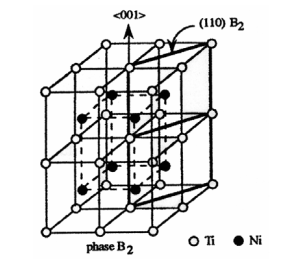
\includegraphics[scale=0.4]{img/B2Phase.png}
				}
				\subfloat[Fase B19'.]{
					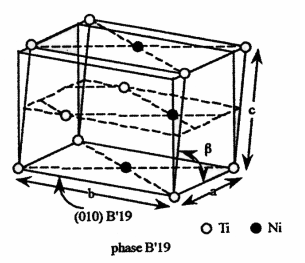
\includegraphics[scale=0.4]{img/B19pPhase.png}
				}
			\end{figure}
		\end{frame}
		\begin{frame}{Termodinámica de la transformación}
			Termo de la transformación
		\end{frame}

\section{Técnicas experimentales}

	\subsection{Deposición por magnetrón sputtering}
		\begin{frame}{Deposición por magnetrón sputtering}
			\begin{figure}[H]
				\subfloat[Esquema magentrón.]{
					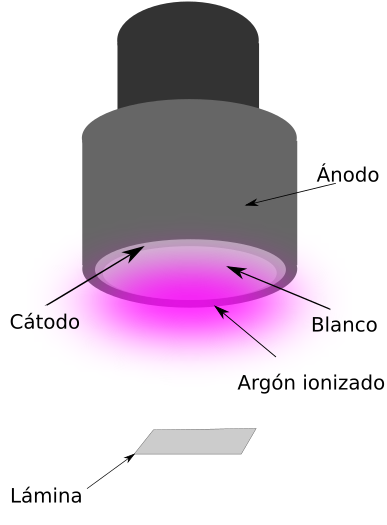
\includegraphics[scale=0.1]{img/SchemaDeposition.png}
				}\qquad
				\subfloat[Magnetrones empleados durante las deposiciones.]{
					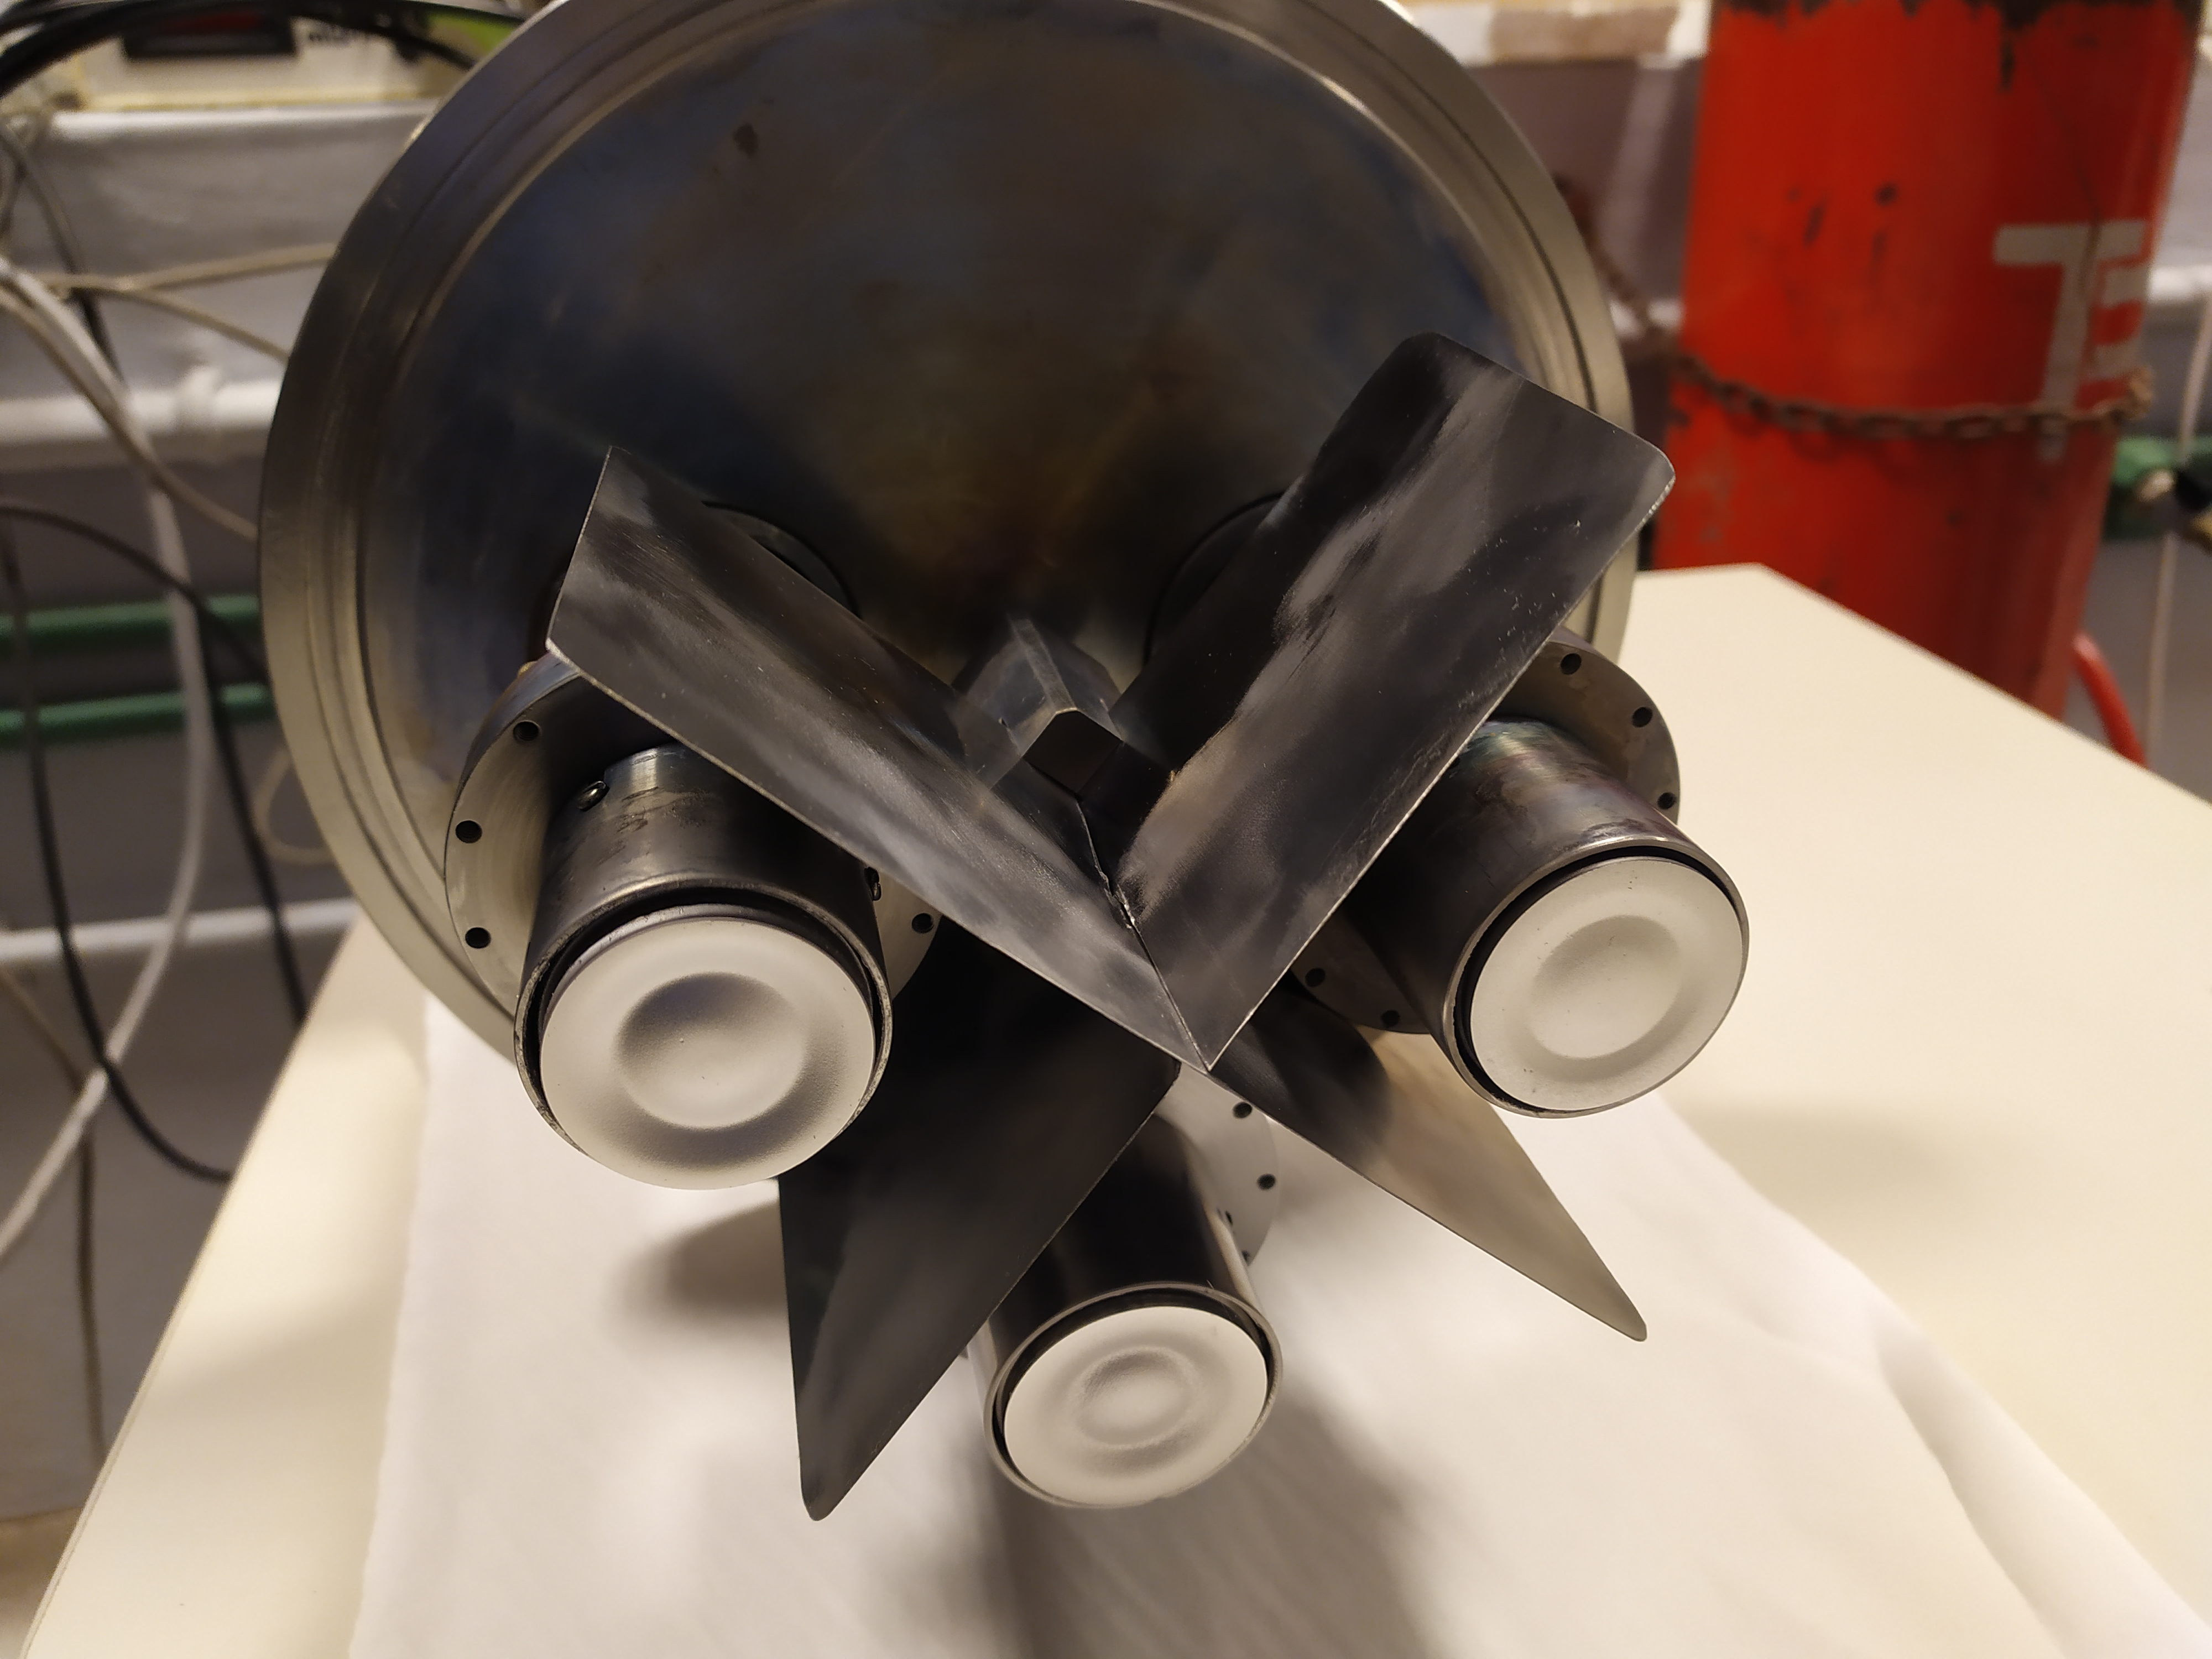
\includegraphics[scale=0.05]{img/magnetrones.jpg}
				}
			\end{figure}
		\end{frame}
	
	\subsection{Microscopía electrónica de barrido}
		\begin{frame}{}
			\begin{figure}[H]
				\centering
				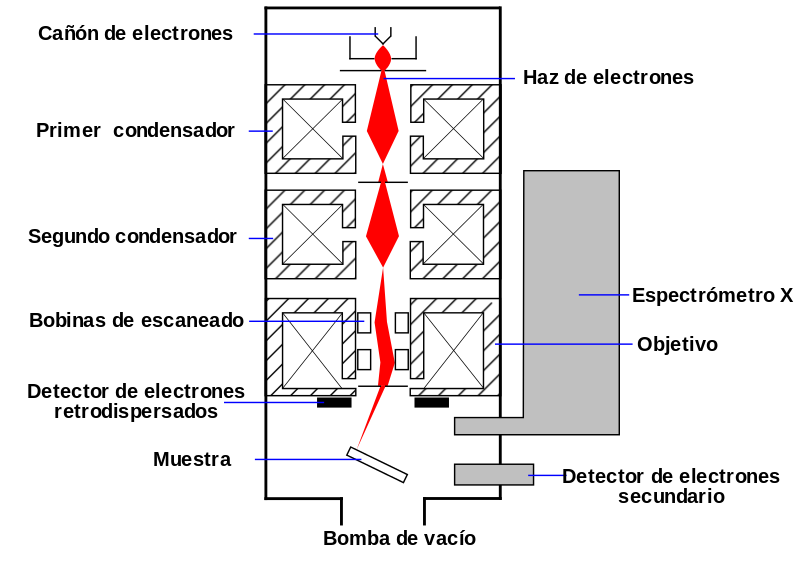
\includegraphics[scale=0.3]{img/SEM.png}
				\caption{Esquema microscopio electrónico de barrido.}
			\end{figure}
		\end{frame}
	
	\subsection{Difracción por rayos X}
		\begin{frame}{}
			\begin{figure}[H]
				\centering
				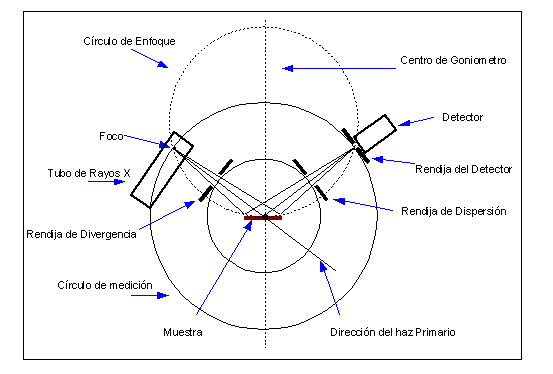
\includegraphics[scale=0.6]{img/gonio.png}
				\caption{Esquema del dispositivo tipo Bragg-Brentano.}
			\end{figure}
		\end{frame}
	
	\subsection{Microscopía electrónica de transmisión}
		\begin{frame}{}
			\begin{figure}[H]
				\centering
				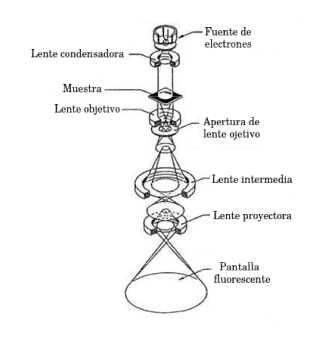
\includegraphics[scale=0.4]{img/TEM.png}
				\caption{Esquema del tubo de un microscopio electrónico de 							  transmisión}
			\end{figure}
		\end{frame}

	\subsection{Calorimetría diferencial de barrido}
		\begin{frame}
			\begin{figure}[H]
				\centering
				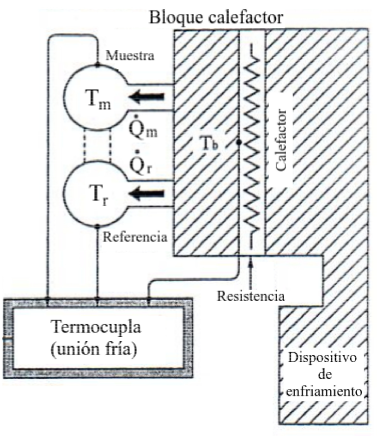
\includegraphics[scale=0.1]{img/DSCscheme.png}
				\caption{Esquema del DSC empleado.}
			\end{figure}
		\end{frame}

	\subsection{Resistividad por el método de cuatro puntas}
		\begin{frame}
			\begin{figure}[H]
				\centering
				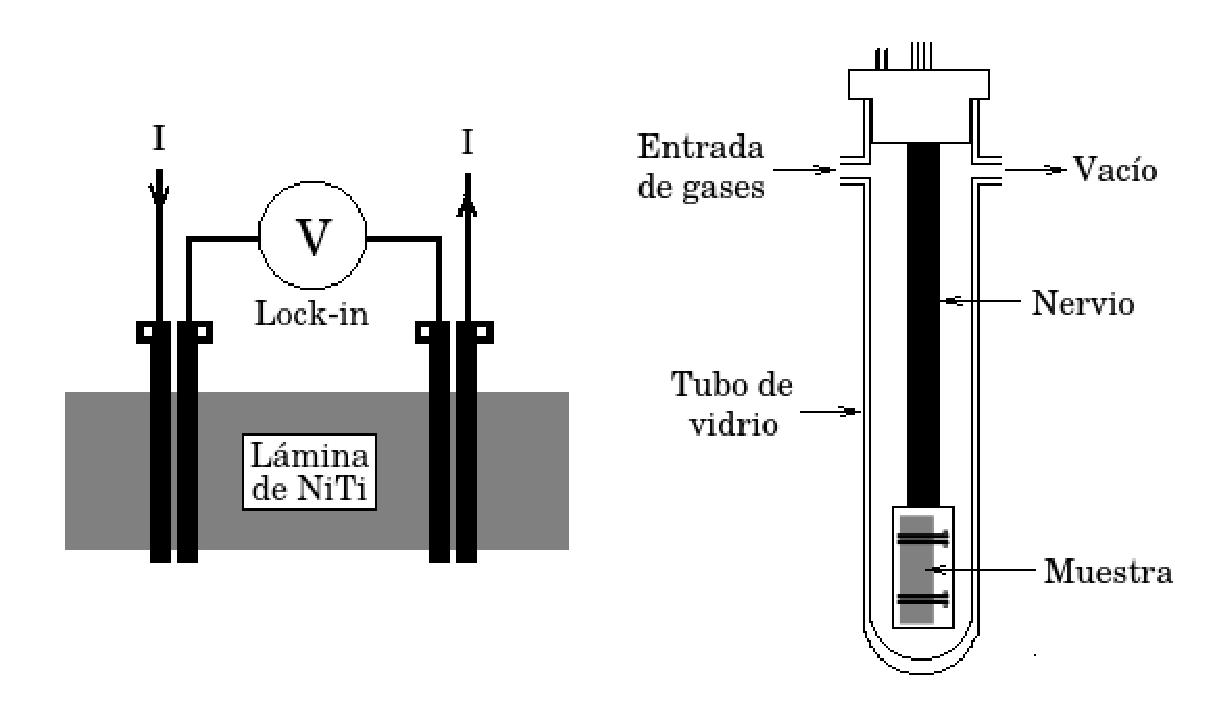
\includegraphics[scale=0.4]{img/resistividad.eps}
				\caption{Esquema del sistema empleado para el método de 								 resistividad por cuatro puntas.}
			\end{figure}
		\end{frame}
	
\section{Resultados obtenidos}
	\subsection{Deposición de las láminas}
		\begin{frame}
			\begin{table}[H]
				\centering
				\begin{tabular}{c|c|c|}
				\cline{2-3}
				\multicolumn{1}{l|}{} & Primera Deposición 2 & Tercera Deposición \\ \hline
				\multicolumn{1}{|c|}{Ti{[}\%at{]}} & 30,8 $\pm$ 0,6 & 33,2 $\pm$ 0,5 \\ \hline
				\multicolumn{1}{|c|}{Ni{[}\%at{]}} & 50,4 $\pm$ 0,2 & 46 $\pm$ 1 \\ \hline
				\multicolumn{1}{|c|}{Zr{[}\%at{]}} & 18,9 $\pm$ 0,5 & 20,8 $\pm$ 0,4 \\ \hline
				\end{tabular}
				\caption{Composición determinada para ambas deposiciones.}
				\label{compositionAvg}
			\end{table}
		\end{frame}

	\subsection{Energía de activación}
	\begin{frame}
		\begin{figure}
			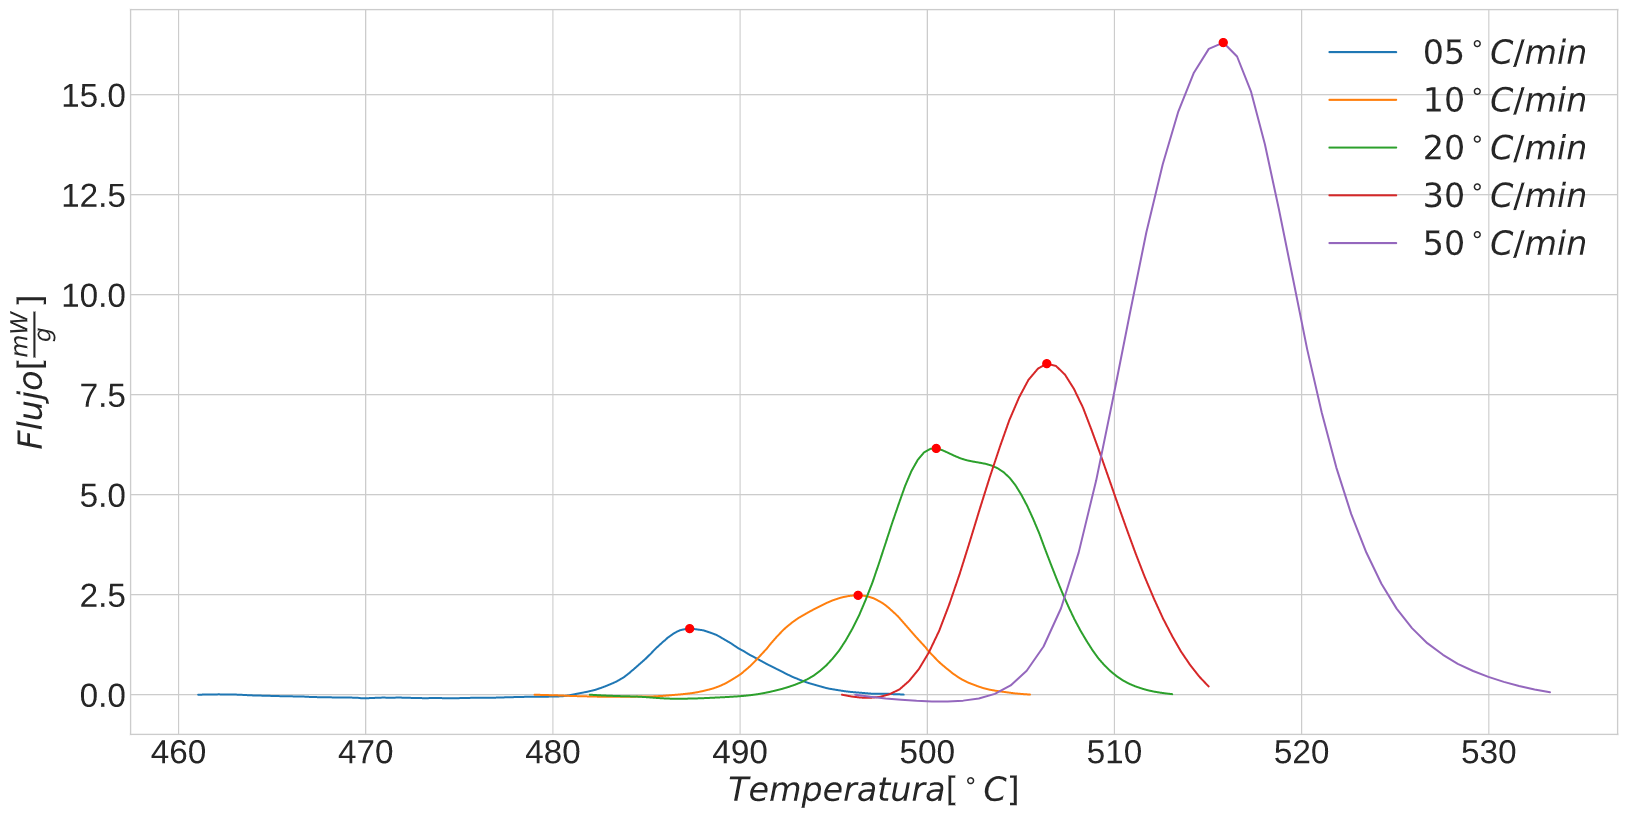
\includegraphics[scale=0.4]{img/DSCPeaks.png}
		\end{figure}
		\begin{figure}
			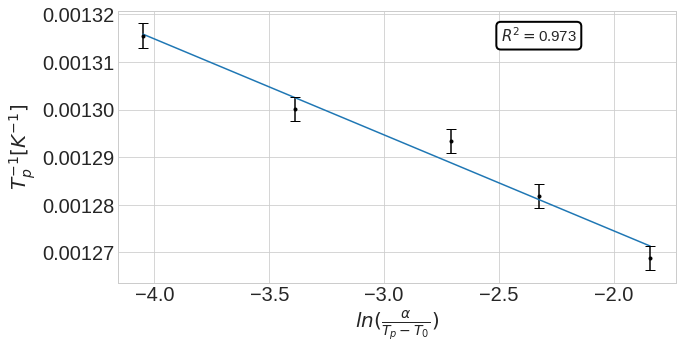
\includegraphics[scale=0.4]{img/Augis_bennet.png}
		\end{figure}
		\begin{figure}
			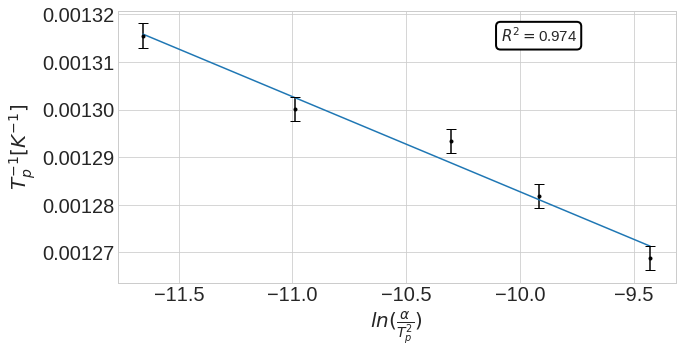
\includegraphics[scale=0.4]{img/Kissinger.png}
		\end{figure}
	\end{frame}

	\subsection{Fases obtenidas}
		\begin{frame}{Pobres en $Ni$}
			\begin{figure}[H]
				\subfloat[Muestra a $500 ^\circ C$]{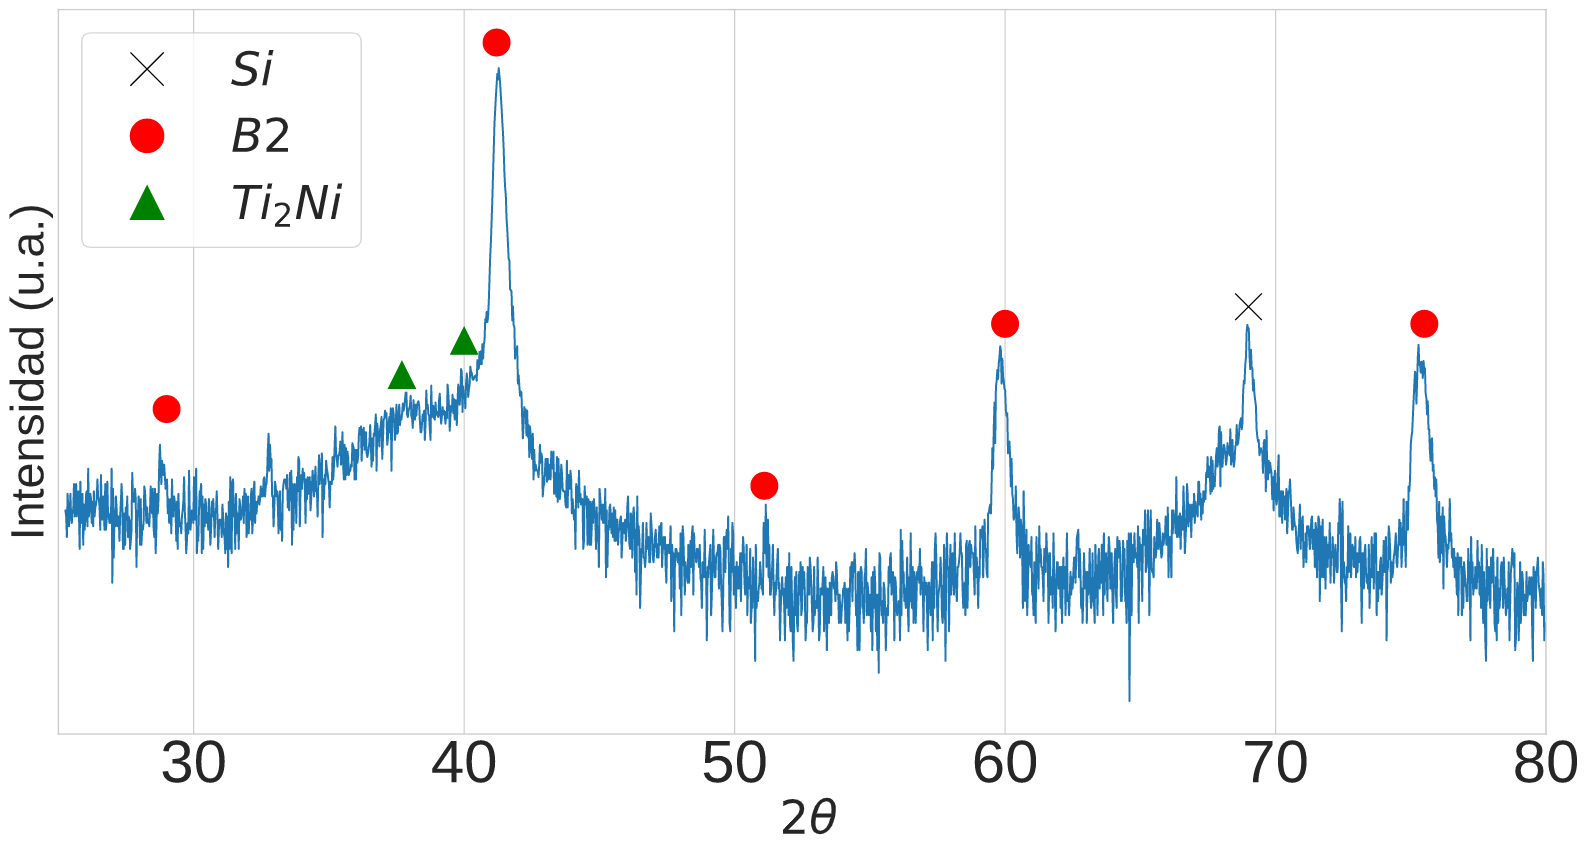
\includegraphics[scale=0.1]{img/RX/NiPoor_500.png}} 
				\subfloat[Muestra a $600 ^\circ C$]{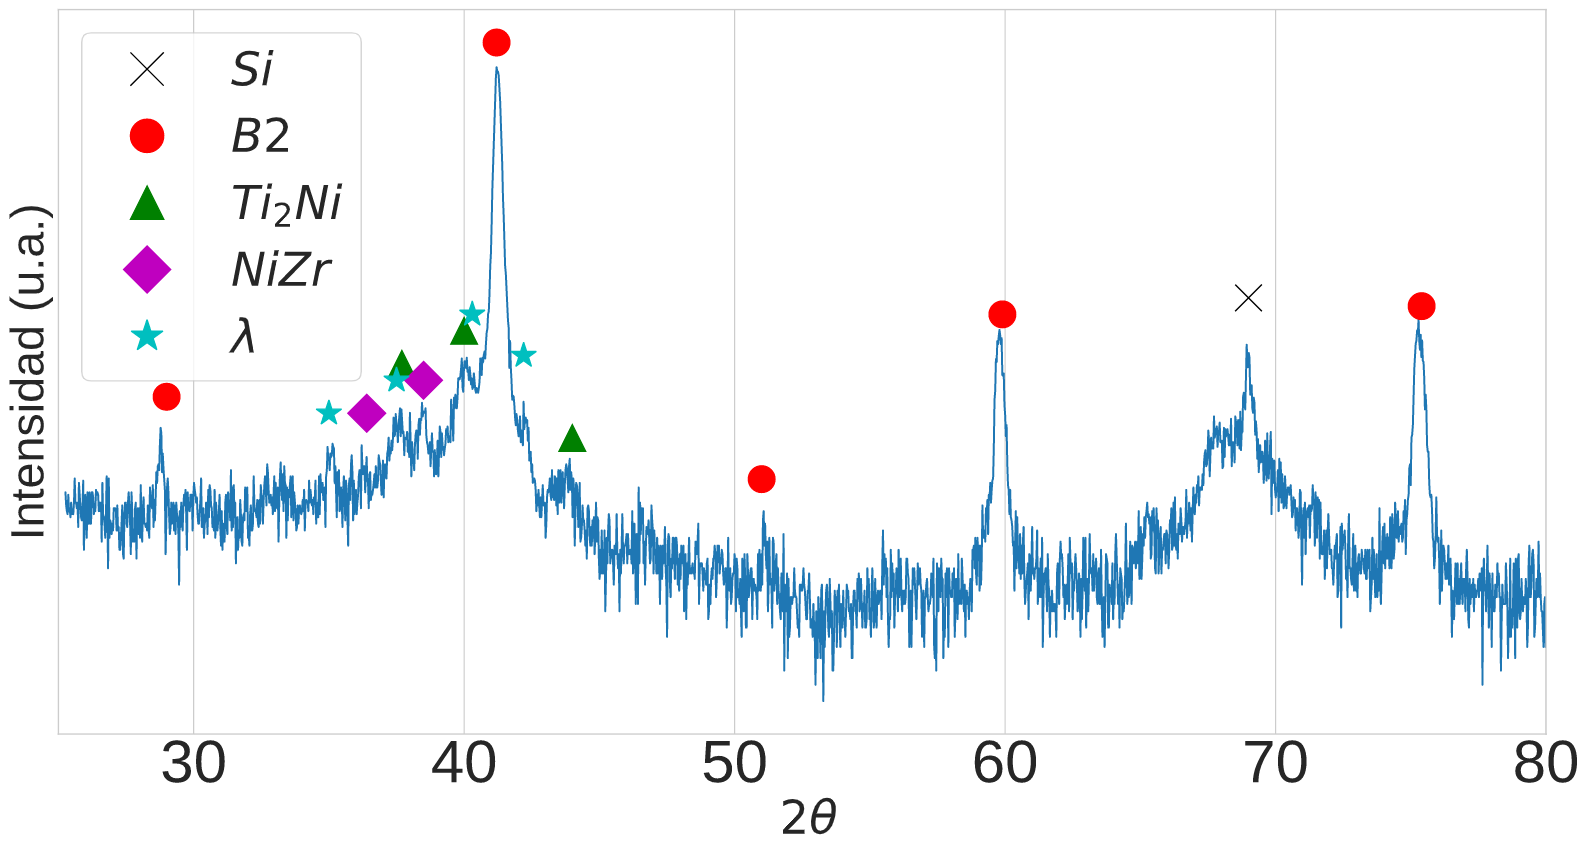
\includegraphics[scale=0.1]{img/RX/NiPoor_600.png}} \\
				\subfloat[Muestra a $700 ^\circ C$]{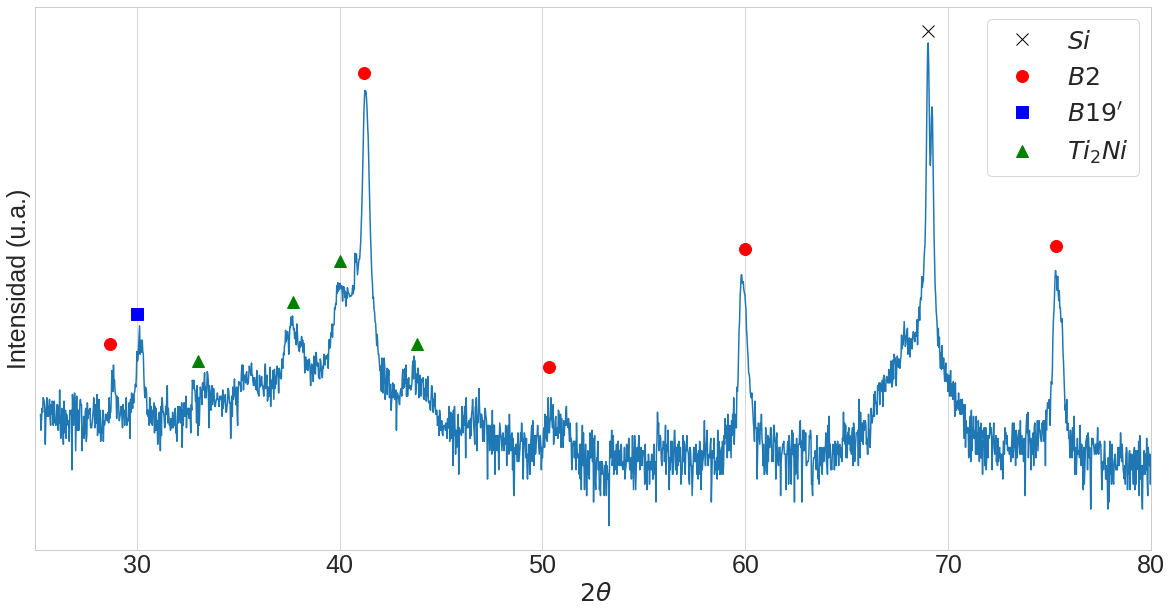
\includegraphics[scale=0.1]{img/RX/NiPoor_700.png}}
				\subfloat[Muestra a $800 ^\circ C$]{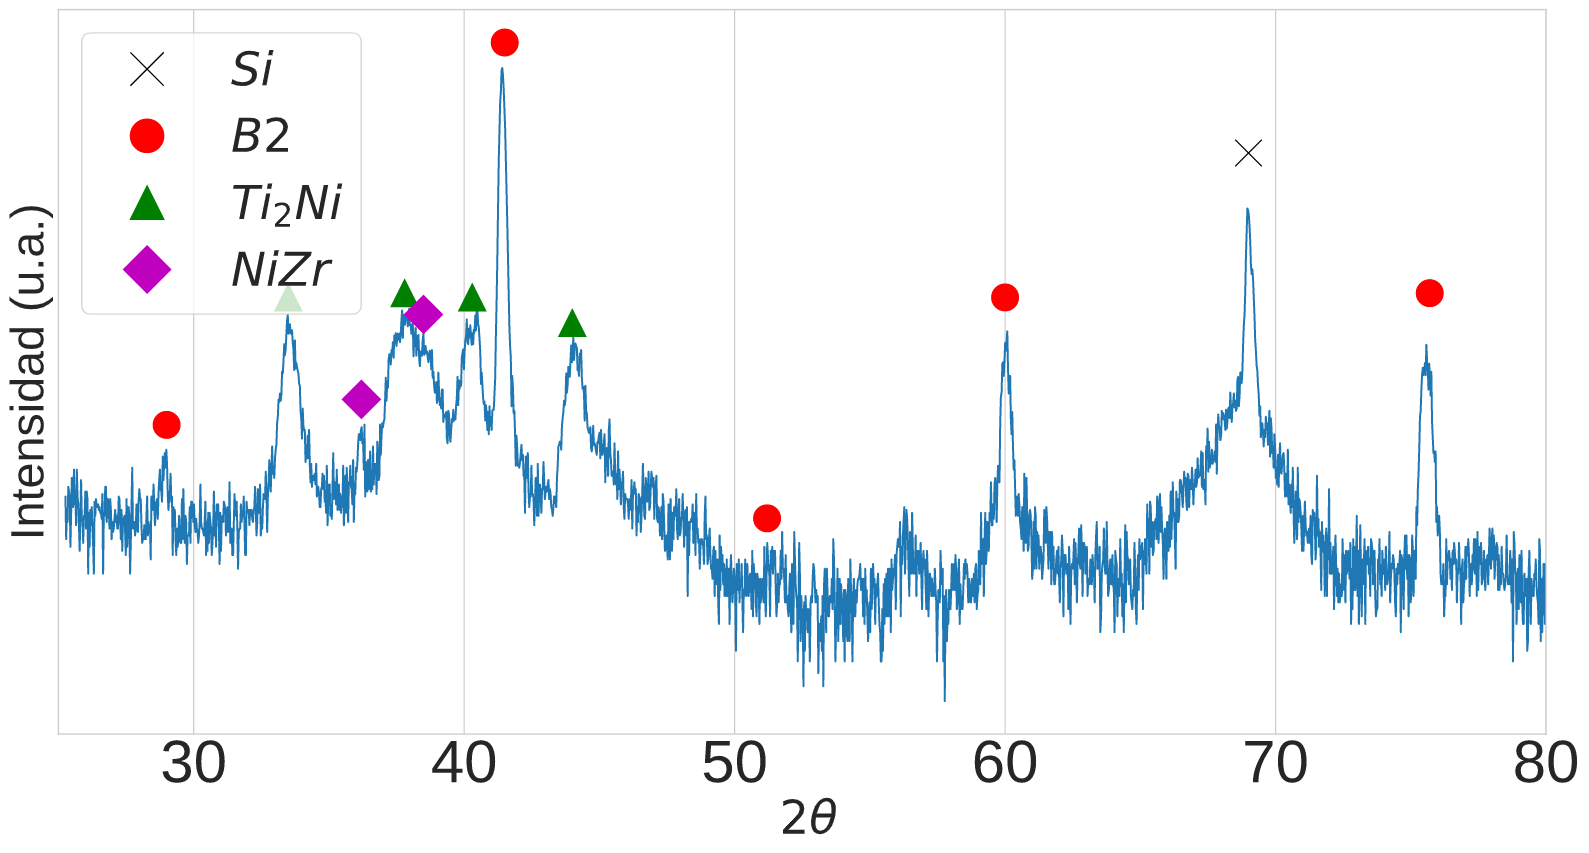
\includegraphics[scale=0.1]{img/RX/NiPoor_800.png}} \\
				\caption{Patrones de difracción para las muestras pobres en $Ni$.}
				\label{RXNiPoor}
			\end{figure}		
		\end{frame}
		
		\begin{frame}{Ricas en $Ni$}
			\begin{figure}[H]
				\subfloat[Muestra a $500 ^\circ C$]{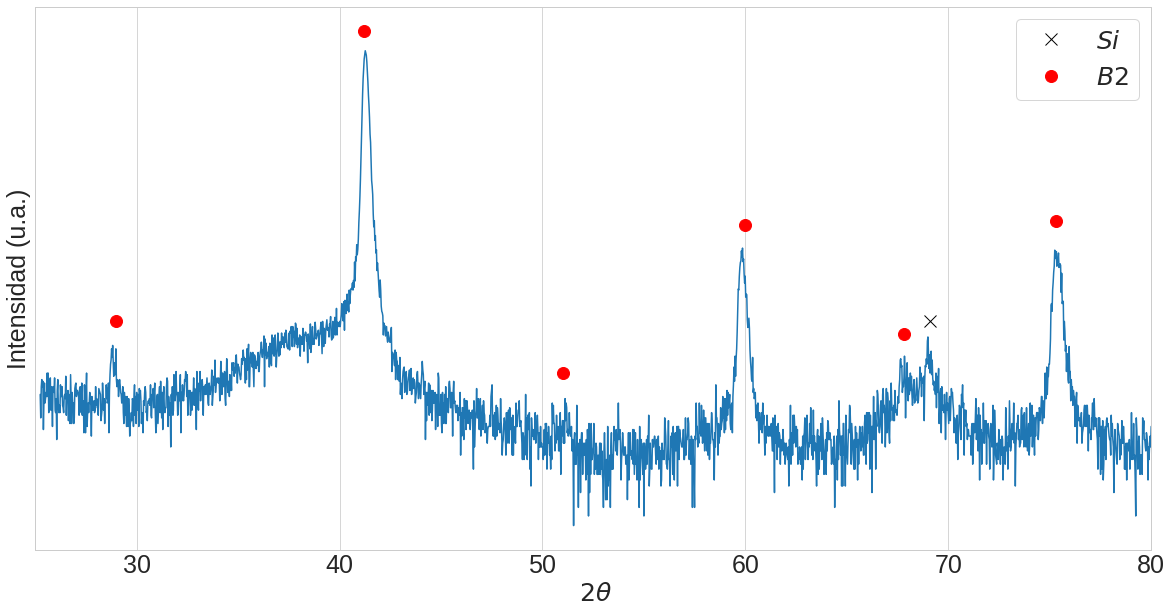
\includegraphics[scale=0.1]{img/RX/NiRich_500.png}} 
				\subfloat[Muestra a $600 ^\circ C$]{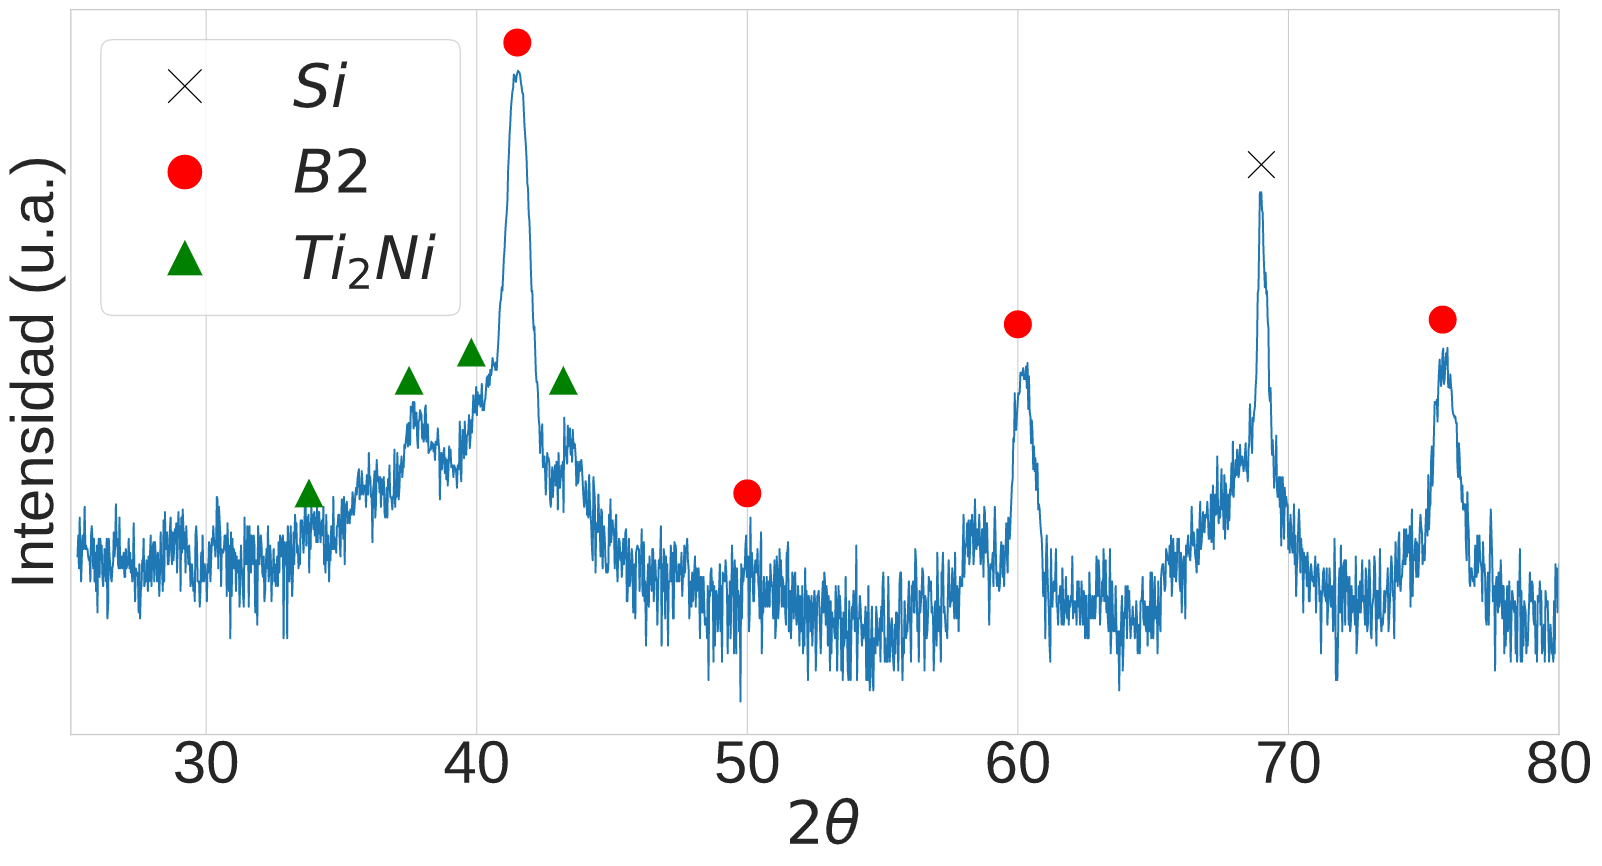
\includegraphics[scale=0.1]{img/RX/NiRich_600.png}} \\
				\subfloat[Muestra a $700 ^\circ C$]{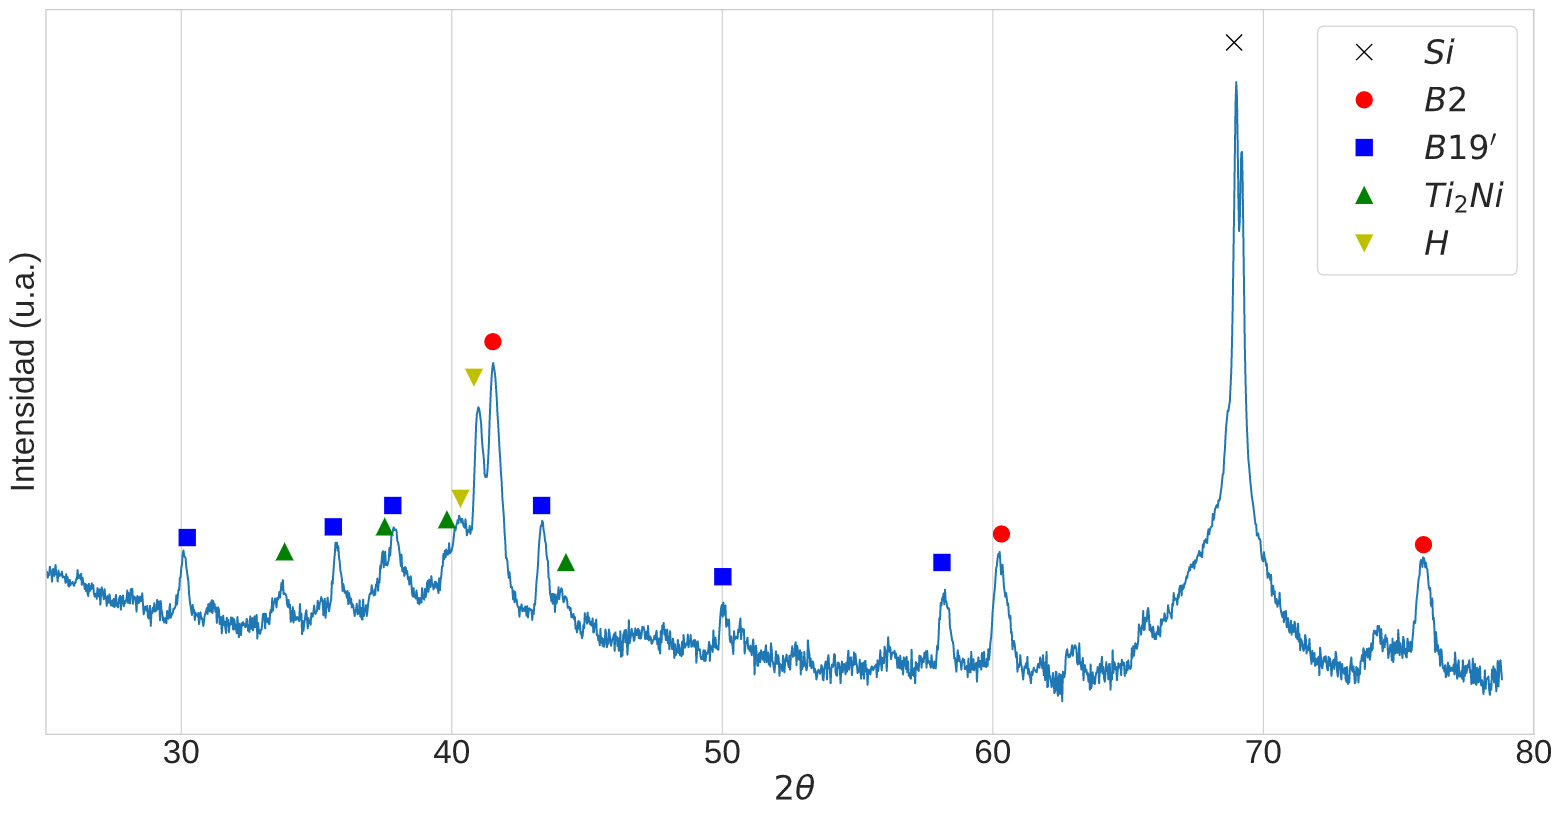
\includegraphics[scale=0.076]{img/RX/NiRich_700.png}}
				\subfloat[Muestra a $800 ^\circ C$]{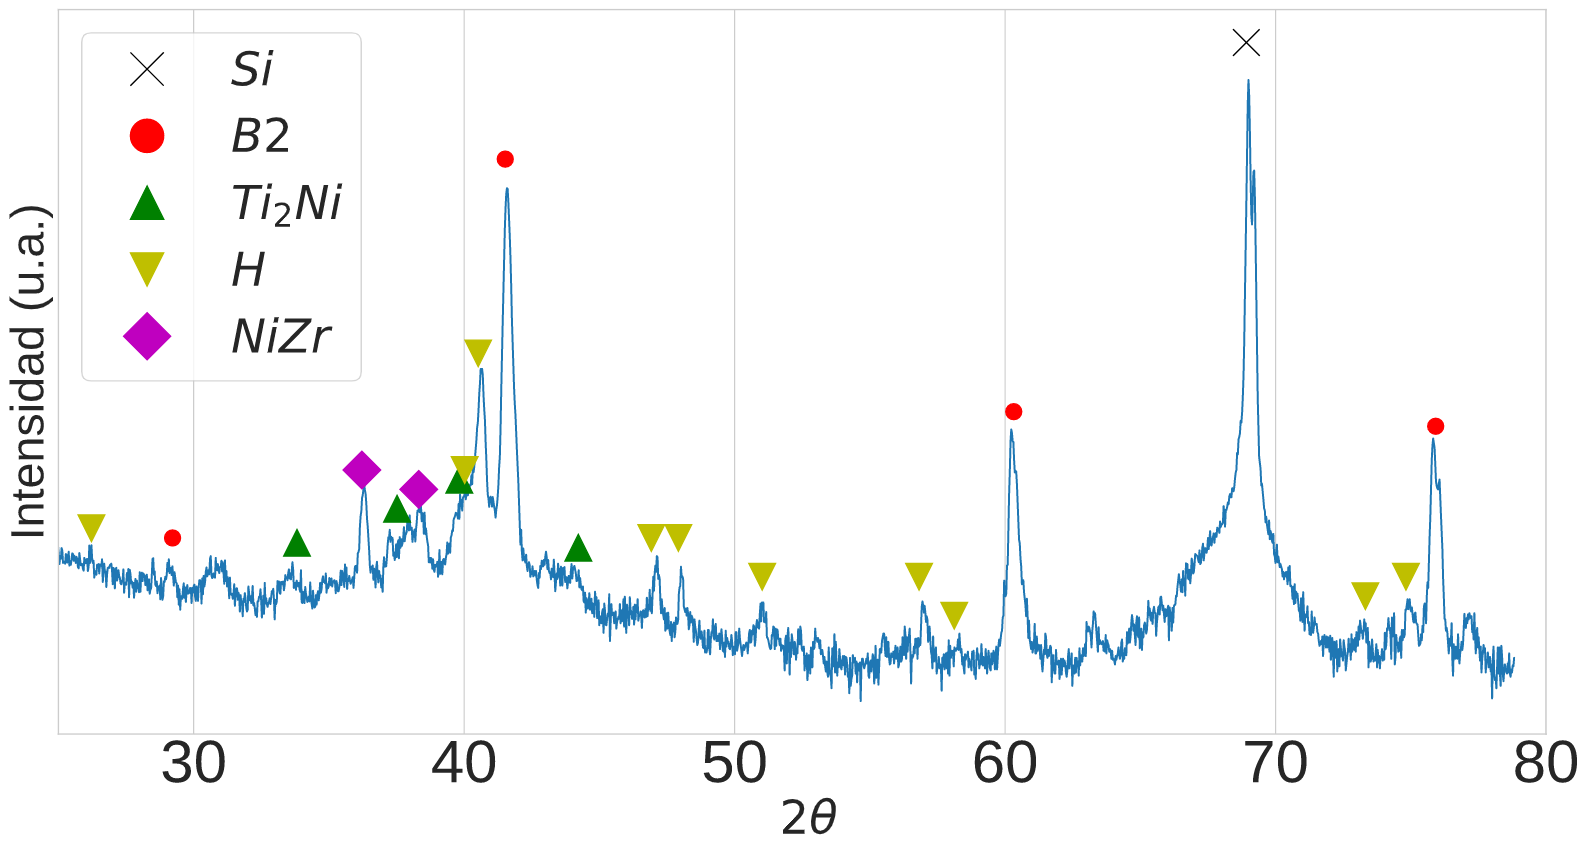
\includegraphics[scale=0.1]{img/RX/NiRich_800.png}} \\
				\caption{Patrones de difracción para las muestras pobres en $Ni$.}
				\label{RXNiRich}
			\end{figure}		
		\end{frame}
	\subsection{Imágenes obtenidas por TEM}
	\subsection{Transformación Martensítica}
\section{Conclusión}

\end{document}
